%definira klasu dokumenta 
\documentclass[12pt]{report} 

%prostor izmedu naredbi \documentclass i \begin{document} se zove uvod. U njemu se nalaze naredbe koje se odnose na cijeli dokument
	
	%osnovni LaTex ne može riješiti sve probleme, pa se koriste različiti paketi koji olakšavaju izradu željenog dokumenta
	\usepackage[croatian]{babel} 
	\usepackage{amssymb}
	\usepackage{amsmath}
	\usepackage{txfonts}
	\usepackage{mathdots}
	\usepackage{titlesec}
	\usepackage{array}
	\usepackage{lastpage}
	\usepackage{etoolbox}
	\usepackage{longtable}[=v4.13]
	\usepackage{tabu}
	\usepackage{color, colortbl}
	\usepackage{adjustbox}
	\usepackage{geometry}
	\usepackage[classicReIm]{kpfonts}
	\usepackage{hyperref}
	\usepackage{fancyhdr}
	
	\usepackage{float}
	\usepackage{setspace}
	\restylefloat{table}
	
	
	\patchcmd{\chapter}{\thispagestyle{plain}}{\thispagestyle{fancy}}{}{} %redefiniranje stila stranice u paketu fancyhdr
	
	%oblik naslova poglavlja
	\titleformat{\chapter}{\normalfont\huge\bfseries}{\thechapter.}{20pt}{\Huge}
	\titlespacing{\chapter}{0pt}{0pt}{40pt}
	
	
	\linespread{1.3} %razmak između redaka
	
	\geometry{a4paper, left=1in, top=1in,}  %oblik stranice
	
	\hypersetup{ colorlinks, citecolor=black, filecolor=black, linkcolor=black,	urlcolor=black }   %izgled poveznice
	
	
	%prored smanjen između redaka u nabrajanjima i popisima
	\newenvironment{packed_enum}{
		\begin{enumerate}
			\setlength{\itemsep}{0pt}
			\setlength{\parskip}{0pt}
			\setlength{\parsep}{0pt}
		}{\end{enumerate}}
	
	\newenvironment{packed_item}{
		\begin{itemize}
			\setlength{\itemsep}{0pt}
			\setlength{\parskip}{0pt}
			\setlength{\parsep}{0pt}
		}{\end{itemize}}
	
	
	%boja za privatni i udaljeni kljuc u tablicama
	\definecolor{LightBlue}{rgb}{0.9,0.9,1}
	\definecolor{LightGreen}{rgb}{0.9,1,0.9}
	
	
	%podesavanje zaglavlja i podnožja
	
	\pagestyle{fancy}
	\lhead{Programsko inženjerstvo}
	\rhead{Radno vrijeme}
	\lfoot{DugonogiProgi}
	\cfoot{stranica \thepage/\pageref{LastPage}}
	\rfoot{\today}
	\renewcommand{\headrulewidth}{0.2pt}
	\renewcommand{\footrulewidth}{0.2pt}
	
	
	\begin{document} 
		
		
		
		\begin{titlepage}
			\begin{center}
				\vspace*{\stretch{1.0}} %u kombinaciji s ostalim \vspace naredbama definira razmak između redaka teksta
				\LARGE Programsko inženjerstvo\\
				\large Ak. god. 2021./2022.\\
				
				\vspace*{\stretch{3.0}}
				
				\huge Radno vrijeme\\
				\Large Dokumentacija, Rev. \textit{0.4}\\
				
				\vspace*{\stretch{12.0}}
				\normalsize
				Grupa: \textit{DugonogiProgi}\\
				Voditelj: \textit{Bernard Kazazić}\\
				
				
				\vspace*{\stretch{1.0}}
				Datum predaje: \textit{17.10.2021.}\\
				
				\vspace*{\stretch{4.0}}
				
				Nastavnik: \textit{Miljenko Krhen}\\
				
			\end{center}
			
			
		\end{titlepage}
		
		
		\tableofcontents
		
		\chapter{Dnevnik promjena dokumentacije}


\begin{longtabu} to \textwidth {|X[2, l]|X[13, l]|X[3, l]|X[3, l]|}
	\hline \multicolumn{1}{|l|}{\textbf{Rev.}}	& \multicolumn{1}{l|}{\textbf{Opis promjene/dodatka}} & \multicolumn{1}{l|}{\textbf{Autori}} & \multicolumn{1}{l|}{\textbf{Datum}} \\[3pt] \hline
	\endfirsthead
	
	\hline \multicolumn{1}{|l|}{\textbf{Rev.}}	& \multicolumn{1}{l|}{\textbf{Opis promjene/dodatka}} & \multicolumn{1}{|l|}{\textbf{Autori}} & \multicolumn{1}{l|}{\textbf{Datum}} \\[3pt] \hline
	\endhead
	
	\hline 
	\endlastfoot
	
	0.1 	& Napravljen predložak.			& Raspudić & 14.10.2021. \\[3pt] \hline 
	0.1.1	& Dopisani dnevnici sastajanja.	& Raspudić & 15.10.2021.	\\[3pt] \hline 
	0.2 	& Dodani nefunkcionalni zahtjevi.  & Raspudić & 16.10.2021. \\[3pt] \hline 
	0.3 	& Dodani funkcionalni zahtjevi.  & Pašalić, Sušac & 17.10.2021. \\[3pt] \hline 
	0.4 	& Dodan opis projekta.  & Pavlović, Raspudić & 21.10.2021. \\[3pt] \hline 
	0.5 	& (1)\newline Dodani obrasci uporabe i sekvencijski dijagrami \newline \newline
			  (2)\newline Dodana arhitektura i dizajn sustava & (1) M.Erlić, A.Pašalić, V.Žunar \newline
			  											(2) B.Kazazić, P.Sušac & 24.10.2021. \\[3pt] \hline 
	0.5.1	 & Manje gramatičke izmjene. & Raspudić & 04.11.2021. \\[3pt] \hline 
	\hline 
	0.6	 & Napravljeni dijagrami razreda. & M. Erlić, B. Pavlović, B. Kazazić, V. Žunar  & 18.11.2021. \\[3pt] \hline 
	\hline 
	0.6.1	 & Opis dijagrama razreda & M. Erlić, B. Pavlović, B. Kazazić, V. Žunar  & 19.11.2021. \\[3pt] \hline 
	1.0	 & Ispravak dijagrama razreda & M. Erlić, B. Pavlović, B. Kazazić, V. Žunar  & 10.12.2021. \\[3pt] \hline
	
	1.1 	& (1)\newline Dodan dijagram stanja \newline \newline
			  (2)\newline Dodan dijagram aktivnosti
			  \newline
			  (3)\newline Dodan dijagram komponenti
			  & (1) B. Pavlović \newline
			  	(2) M. Erlić\newline
			  		(3) M. Erlić, L. Raspudić, A. Pašalić
			  		& 20.12.2021. \\[3pt] \hline
    1.2 	& (1)\newline Opis korištenih tehnologija i alata \newline \newline
			  (2)\newline Prikaz ispitivanja komponenata
			  \newline
			  (3)\newline Ispitivanje sustava (Selenium IDE)
			  \newline
			  (4)\newline Dodan dijagram razmještaja
			  & (1) B. Pavlović, V. Žunar \newline
			  	(2) M. Erlić, B. Pavlović\newline
			  		(3) P. Sušac\newline
			  		(4) V. Žunar
			  		& 4.1.2022. \\[3pt] \hline
	1.3 	& Stvorene upute za puštanje u pogon
			  & B. Kazazić 
			  		& 6.1.2022. \\[3pt] \hline
    1.4 	& Zaključak i budući rad
			  & V. Žunar
			  		& 7.1.2022. \\[3pt] \hline
    1.5 	& Dodan popis literature
			  & V. Žunar
			  		& 8.1.2022. \\[3pt] \hline
    1.6 	& Dodan dnevnik sastajanja
			  & V. Žunar
			  		& 10.1.2022. \\[3pt] \hline
	1.7 	& Tablica aktivnosti popunjena
			  & V. Žunar, B. Pavlović, L. Raspudić, B. Kazazić, M. Erlić, A. Pašalić
			  		& 11.1.2022. \\[3pt] \hline
	1.8 	& Dodani dijagrami pregleda promjena
			  & B. Kazazić
			  		& 14.1.2022. \\[3pt] \hline
    2.0 	& Završno uređivanje dokumentacije
			  & A. Pašalić
			  		& 14.1.2022. \\[3pt] \hline
	%0.9 & Opisi obrazaca uporabe & Jović & 07.09.2013. \\[3pt] \hline 
	%0.10 & Preveden uvod & Jović & 08.09.2013. \\[3pt] \hline 
	%0.11 & Sekvencijski dijagrami & Žužak & 09.09.2013. \\[3pt] \hline 
	%0.12.1 & Započeo dijagrame razreda & Horvat & 10.09.2013. \\[3pt] \hline 
	%0.12.2 & Nastavak dijagrama razreda & Horvat & 11.09.2013. \\[3pt] \hline 
	%\textbf{1.0} & Verzija samo s bitnim dijelovima za 1. ciklus & Ivošević & 11.09.2013. \\[3pt] \hline 
	%1.1 & Uređivanje teksta -- funkcionalni i nefunkcionalni zahtjevi & Grudenić \newline Jović & %14.09.2013. \\[3pt] \hline 
	%1.2 & Manje izmjene:Timer - Brojilo vremena & Grudenić & 15.09.2013. \\[3pt] \hline 
	%1.3 & Popravljeni dijagrami obrazaca uporabe & Jović & 15.09.2013. \\[3pt] \hline 
	%1.5 & Generalna revizija strukture dokumenta & Ivošević & 19.09.2013. \\[3pt] \hline 
	%1.5.1 & Manja revizija (dijagram razmještaja) & Jović & 20.09.2013. \\[3pt] \hline 
	%\textbf{2.0} & Konačni tekst predloška dokumentacije  & Ivošević & 28.09.2013. \\[3pt] \hline 
	%&  &  & \\[3pt] \hline
	
	
\end{longtabu}


%\textit{Moraju postojati glavne revizije dokumenata 1.0 i 2.0 na kraju prvog i drugog ciklusa. Između tih revizija mogu postojati manje revizije već prema tome kako se dokument bude nadopunjavao. Očekuje se da nakon svake značajnije promjene (dodatka, izmjene, uklanjanja dijelova teksta i popratnih grafičkih sadržaja) dokumenta se to zabilježi kao revizija. Npr., revizije unutar prvog ciklusa će imati oznake 0.1, 0.2, …, 0.9, 0.10, 0.11.. sve do konačne revizije prvog ciklusa 1.0. U drugom ciklusu se nastavlja s revizijama 1.1, 1.2, itd.}
		\chapter{Opis projektnog zadatka}
		
		\textbf{\textit{dio 1. revizije}}\\
		
		\textit{Na osnovi projektnog zadatka detaljno opisati korisničke zahtjeve. Što jasnije opisati cilj projektnog zadatka, razraditi problematiku zadatka, dodati nove aspekte problema i potencijalnih rješenja. Očekuje se minimalno 3, a poželjno 4-5 stranica opisa.	Teme koje treba dodatno razraditi u ovom poglavlju su:}
		\begin{packed_item}
			\item \textit{potencijalna korist ovog projekta}
			\item \textit{postojeća slična rješenja (istražiti i ukratko opisati razlike u odnosu na zadani zadatak). Dodajte slike koja predočavaju slična rješenja.}
			\item \textit{skup korisnika koji bi mogao biti zainteresiran za ostvareno rješenje.}
			\item \textit{mogućnost prilagodbe rješenja }
			\item \textit{opseg projektnog zadatka}
			\item \textit{moguće nadogradnje projektnog zadatka}
		\end{packed_item}
		
		\textit{Za pomoć pogledati reference navedene u poglavlju „Popis literature“, a po potrebi konzultirati sadržaj na internetu koji nudi dobre smjernice u tom pogledu.}
		\eject
		
		%\section{Primjeri u \LaTeX u}
		
		%\textit{Ovo potpoglavlje izbrisati.}\\

		%U nastavku se nalaze različiti primjeri kako koristiti osnovne funkcionalnosti \LaTeX a koje su potrebne za izradu dokumentacije. Za dodatnu pomoć obratiti se asistentu na projektu ili potražiti upute na sljedećim web sjedištima:
		%\begin{itemize}
			%\item Upute za izradu diplomskog rada u \LaTeX u - \url{https://www.fer.unizg.hr/_download/repository/LaTeX-upute.pdf}
			%\item \LaTeX\ projekt - \url{https://www.latex-project.org/help/}
			%\item StackExchange za Tex - %\url{https://tex.stackexchange.com/}\\
		
		%\end{itemize} 	


		
		%\noindent \underbar{podcrtani tekst}, \textbf{podebljani tekst}, 	\textit{nagnuti tekst}\\
		%\noindent \normalsize primjer \large primjer \Large primjer \LARGE {primjer} \huge {primjer} \Huge primjer \normalsize
				
		%\begin{packed_item}
			
			%\item  primjer
			%\item  primjer
			%\item  primjer
			%\item[] \begin{packed_enum}
			%	\item primjer
			%	\item[] \begin{packed_enum}
			%		\item[1.a] primjer
			%		\item[b] primjer
			%	\end{packed_enum}
			%	\item primjer
			%\end{packed_enum}
			
		%\end{packed_item}
		
		%\noindent primjer url-a: \url{https://www.fer.unizg.hr/predmet/proinz/projekt}
		
		%\noindent posebni znakovi: \# \$ \% \& \{ \} \_ 
		%$|$ $<$ $>$ 
		%\^{} 
		%\~{} 
		%$\backslash$ 
		
		%\begin{longtabu} to \textwidth {|X[8, l]|X[8, l]|X[16, l]|} %definicija širine tablice, širine stupaca i poravnanje
			
		%	%definicija naslova tablice
		%	\hline \multicolumn{3}{|c|}{\textbf{naslov unutar tablice}}	 \\[3pt] \hline
		%	\endfirsthead
			
			%definicija naslova tablice prilikom prijeloma
		%	\hline \multicolumn{3}{|c|}{\textbf{naslov unutar tablice}}	 \\[3pt] \hline
		%	\endhead
			
		%	\hline 
		%	\endlastfoot
			
		%	\rowcolor{LightGreen}IDKorisnik & INT	&  	Lorem ipsum dolor sit amet, consectetur adipiscing elit, sed do eiusmod  	\\ \hline
		%	korisnickoIme	& VARCHAR &   	\\ \hline 
		%	email & VARCHAR &   \\ \hline 
		%	ime & VARCHAR	&  		\\ \hline 
		%	\cellcolor{LightBlue} primjer	& VARCHAR &   	\\ \hline 
			
		%\end{longtabu}
		

		%\begin{table}[H]
			
		%	\begin{longtabu} to \textwidth {|X[8, l]|X[8, l]|X[16, l]|} 
				
		%		\hline 
		%		\endfirsthead
				
		%		\hline 
		%		\endhead
				
		%		\hline 
		%		\endlastfoot
				
		%		\rowcolor{LightGreen}IDKorisnik & INT	&  	Lorem ipsum dolor sit amet, consectetur adipiscing elit, sed do eiusmod  	\\ \hline
		%		korisnickoIme	& VARCHAR &   	\\ \hline 
		%		email & VARCHAR &   \\ \hline 
		%		ime & VARCHAR	&  		\\ \hline 
		%		\cellcolor{LightBlue} primjer	& VARCHAR &   	\\ \hline 
				
				
		%	\end{longtabu}
	
		%	\caption{\label{tab:referencatablica} Naslov ispod tablice.}
		%\end{table}
		
		
		%unos slike
		%\begin{figure}[H]
		%	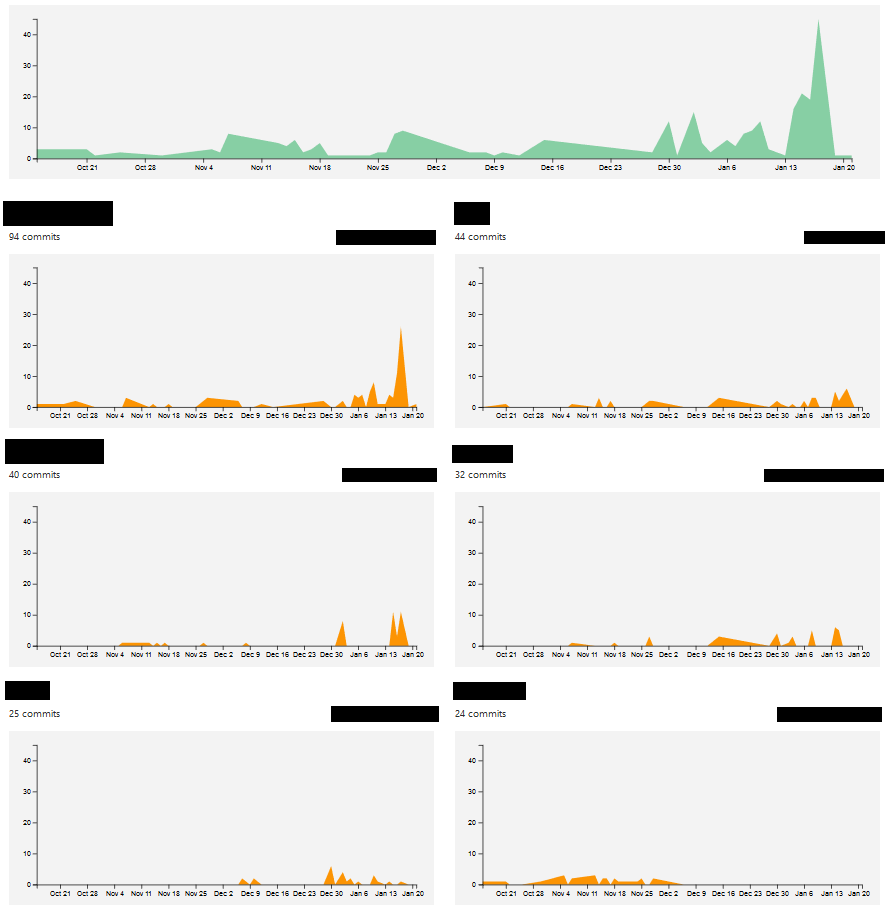
\includegraphics[scale=0.4]{slike/aktivnost.PNG} %veličina slike u odnosu na originalnu datoteku i pozicija slike
		%	\centering
		%	\caption{Primjer slike s potpisom}
		%	\label{fig:promjene}
		%\end{figure}
		
		%\begin{figure}[H]
		%	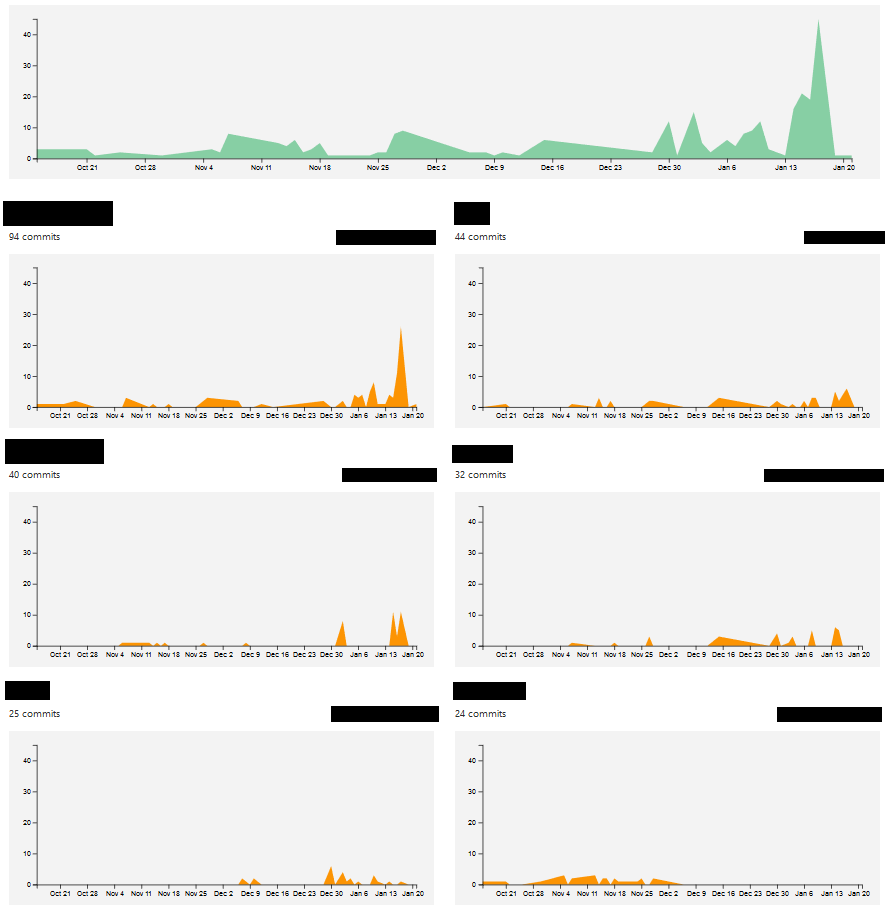
\includegraphics[width=.9\linewidth]{slike/aktivnost.PNG} %veličina u odnosu na širinu linije
		%	\caption{Primjer slike s potpisom 2}
		%	\label{fig:promjene2} %label mora biti drugaciji za svaku sliku
		%\end{figure}
		
		%Referenciranje slike \ref{fig:promjene2} u tekstu.
		
		\eject
		
	
		\chapter{Specifikacija programske potpore}
		
	\section{Funkcionalni zahtjevi}
			
			
			\noindent \textbf{\\Dionici:}
			
			\begin{packed_enum}
				\item Vlasnik sustava (direktor poduzeća/naručitelj)
				\item Djelatnici poduzeća
				\begin{itemize}
					\item Voditelji grupa
					\item Ostali djelatnici
				\end{itemize}
				\item Razvojni tim
			\end{packed_enum}
			
			\noindent \textbf{Aktori i njihovi funkcionalni zahtjevi:}
			\begin{packed_enum}
				\item  \underbar{Vlasnik sustava (direktor poduzeća) može:}
				
				\begin{packed_enum}
					\item definirati uslužne djelatnosti koje će poduzeće raditi
					\item dodijeliti djelatnosti voditeljima grupa
					\item registrirati novog djelatnika (uključujući i voditelja grupa) i pritom mu dodijeliti ulogu
					\item vidjeti zauzetost i realizaciju za sve djelatnike
					\item vidjeti trenutno i prošlu poticiju svih djelatnika koji su izašli na intervencije na karti
				\end{packed_enum}
			
				\item  \underbar{Voditelji grupa mogu:}
				
				\begin{packed_enum}
					\item definirati zadatke i dodjeljivati ih djelatnicima
					\item zabilježiti procjenu radnih sati potrebnih za zadatak
					\item odrediti cijenu sata rada ovisno o djelatnosti ili zadatku
					\item pregledati podatke za sebe i svoju grupu
					\item upisati broj odrađenih sati za svaki dan
				\end{packed_enum}
				\eject
				\item  \underbar{Ostali djelatnici mogu:}
				\begin{packed_enum}
					\item vidjeti koji su mu zadaci dodijeljeni i u kojim se grupama nalazi
					\item pregledati vlastite podatke
					\item upisati broj odrađenih radnih sati za svaki dan
				\end{packed_enum}
			
			\item  \underbar{Neregistrirani korisnik može:}
			\begin{packed_enum}
				\item vidjeti popis i opis djelatnosti poduzeća
			\end{packed_enum}
			\end{packed_enum}
			
			\eject 

			\subsection{Obrasci uporabe}
				
				
				\subsubsection{Opis obrazaca uporabe}
					\textit{Funkcionalne zahtjeve razraditi u obliku obrazaca uporabe. Svaki obrazac je potrebno razraditi prema donjem predlošku. Ukoliko u nekom koraku može doći do odstupanja, potrebno je to odstupanje opisati i po mogućnosti ponuditi rješenje kojim bi se tijek obrasca vratio na osnovni tijek.}\\
					

					\noindent \underbar{\textbf{UC$<$broj obrasca$>$ -$<$ime obrasca$>$}}
					\begin{packed_item}
	
						\item \textbf{Glavni sudionik: }$<$sudionik$>$
						\item  \textbf{Cilj:} $<$cilj$>$
						\item  \textbf{Sudionici:} $<$sudionici$>$
						\item  \textbf{Preduvjet:} $<$preduvjet$>$
						\item  \textbf{Opis osnovnog tijeka:}
						
						\item[] \begin{packed_enum}
	
							\item $<$opis korak jedan$>$
							\item $<$opis korak dva$>$
							\item $<$opis korak tri$>$
							\item $<$opis korak četiri$>$
							\item $<$opis korak pet$>$
						\end{packed_enum}
						
						\item  \textbf{Opis mogućih odstupanja:}
						
						\item[] \begin{packed_item}
	
							\item[2.a] $<$opis mogućeg scenarija odstupanja u koraku 2$>$
							\item[] \begin{packed_enum}
								
								\item $<$opis rješenja mogućeg scenarija korak 1$>$
								\item $<$opis rješenja mogućeg scenarija korak 2$>$
								
							\end{packed_enum}
							\item[2.b] $<$opis mogućeg scenarija odstupanja u koraku 2$>$
							\item[3.a] $<$opis mogućeg scenarija odstupanja  u koraku 3$>$
							
						\end{packed_item}
					\end{packed_item}
				
					
				\subsubsection{Dijagrami obrazaca uporabe}
					
					\textit{Prikazati odnos aktora i obrazaca uporabe odgovarajućim UML dijagramom. Nije nužno nacrtati sve na jednom dijagramu. Modelirati po razinama apstrakcije i skupovima srodnih funkcionalnosti.}
				\eject		
				
			\subsection{Sekvencijski dijagrami}
				
				\textbf{\textit{dio 1. revizije}}\\
				
				\textit{Nacrtati sekvencijske dijagrame koji modeliraju najvažnije dijelove sustava (max. 4 dijagrama). Ukoliko postoji nedoumica oko odabira, razjasniti s asistentom. Uz svaki dijagram napisati detaljni opis dijagrama.}
				\eject
	
		\section{Ostali zahtjevi}
		 	
		 	\noindent Sustav treba:
			 \begin{itemize}
			 	\item omogućiti korištenje hrvatskih dijakritičkih znakova pri unosu i prikazu tekstualnog sadržaja
			 	\item podržati višekorisnički rad u realnom vremenu
			 	\item dati odgovor na traženi upit unutar nekoliko sekundi kada se dohvaćaju podaci iz baze podataka
			 	\item imati intuitivno i jednostavno za korištenje korisničko sučelje
			 	\item biti implementiran kao web aplikacija koristeći objektno-orijentirane jezike
			 	\item neispravno korištenje korisničkog sučelja ne smije narušiti rad sustava
			 	\item osigurati sigurnu, brzu i otpornu na vanjske greške vezu s bazom podataka
			 \end{itemize}
			 
			 
			 
	
		\chapter{Arhitektura i dizajn sustava}
		
	Arhitektura se može podijeliti na tri podsustava: 
	\begin{itemize}
		\item Web poslužitelj 
		\item Web aplikacija 
		\item Baza podataka 
	\end{itemize}
	Web preglednik je program koji korisniku omogućuje pregled web stranica i multimedijalnih sadržaja vezanih uz njih. Svaki internetski preglednik je prevoditelj. Dakle, stranica je pisana u kodu koji preglednik nakon toga interpretira kako nešto svakome razumljivo. Korisnik putem web preglednika šalje zahtjev web poslužitelju. 
	
	Web poslužitelj osnova je rada web aplikacije. Njegova primarna zadaća je komunikacija klijenta s aplikacijom. Komunikacija se odvija preko HTTP (engl. Hyper Text Transfer Protocol) protokola, što je protokol u prijenosu informacija na webu. Poslužitelj je onaj koji pokreće web aplikaciju te joj prosljeđuje zahtjev. 
	
	Korisnik koristi web aplikaciju za obrađivanje željenih zahtjeva. Web aplikacija obrađuje zahtjev te ovisno o zahtjevu, pristupa bazi podataka nakon čega preko poslužitelja vraća korisniku odgovor u obliku HTML dokumenta vidljivog u web pregledniku. 
	
	Programski jezik kojeg smo odabrali za izradu naše web aplikacije je Java Spring Boot. Odabrano razvojno okruženje je Eclipse IDE. Arhitektura sustava temeljiti će se na MVC (Model-View-Controller) konceptu. 
	
	Karakteristika MVC koncepta je nezavisan razvoj pojedinih dijelova aplikacije što za posljedicu ima jednostavnije ispitivanje kao i jednostavnije razvijanje i dodavanje novih svojstava u sustav. \\
	
	MVC koncept sastoji se od: 
	\begin{itemize}
		\item Model - Središnja komponenta sustava. Predstavlja dinamičke strukture podataka, neovisne o korisničkom sučelju. Izravno upravlja podacima, logikom i pravilima aplikacije. Također prima ulazne podatke od Controllera 
		\item View - Bilo kakav prikaz podataka, poput grafa. Mogući su različiti prikazi iste informacije poput grafičkog ili tabličnog prikaza podatak. 
		\item Controller – Prima ulaze i prilagođava ih za prosljeđivanje Model-u ili View-u. Upravlja korisničkim zahtjevima i na temelju njih izvodi daljnju interakciju s ostalim elementima sustava. 
	\end{itemize}
		

		

				
		\section{Baza podataka}
			
			\textbf{\textit{dio 1. revizije}}\\
			
		%\textit{Potrebno je opisati koju vrstu i implementaciju baze podataka ste odabrali, glavne komponente od kojih se sastoji i slično.}
		Baza podataka je predstavljena pomoću ER te relacijskog dijagrama. Od glavnih komponenti, primarno se pojavljuju:
		\begin{itemize}
		\item Employee
		\item Role
		\item Group
		\item EmployeeGroup
		\item Job
		\item Task
		\item EmployeeTask
		\item Location
		\item WorkHoursInput
	    \end{itemize}
		
			\subsection{Opis tablica}
			

				%\textit{Svaku tablicu je potrebno opisati po zadanom predlošku. Lijevo se nalazi točno ime varijable u bazi podataka, u sredini se nalazi tip podataka, a desno se nalazi opis varijable. Svjetlozelenom bojom označite primarni ključ. Svjetlo plavom označite strani ključ}
				
				\subsubsection{Employee}
					Sadrži podatke o djelatniku, uključujući osobne podatke i podatke za prijavu (korisničko ime i lozinka).
				
					\begin{longtabu} to \textwidth {|X[6, l]|X[6, l]|X[20, l]|}
						
						\hline \multicolumn{3}{|c|}{\textbf{Employee}}	 \\[3pt] \hline
						\endfirsthead
						
						\hline \multicolumn{3}{|c|}{\textbf{Employee}}	 \\[3pt] \hline
						\endhead
						
						\hline 
						\endlastfoot

						\cellcolor{LightGreen}pid & CHAR & Osobni identifikacijski broj djelatnika.		\\ \hline
						name	& VARCHAR & Ime djelatnika.  	\\ \hline 
						surname & VARCHAR & Prezime djelatnika.  \\ \hline 
						email & VARCHAR & E-mail adresa.		\\ \hline
						username & VARCHAR	& Jedinstveno korisničko ime djelatnika.	\\ \hline
						password & VARCHAR & Lozinka djelatnika.		\\ \hline   
						\cellcolor{LightBlue} idRole & INTEGER & Identifikator uloge djelatnika. 	\\ \hline 
						
						
					\end{longtabu}

				\subsubsection{Role}
					Sadrži podatke o ulozi korisnika. Uloga može biti: direktor, vođa tima ili djelatnik.
					
					\begin{longtabu} to \textwidth {|X[6, l]|X[6, l]|X[20, l]|}
						
						\hline \multicolumn{3}{|c|}{\textbf{Role}}	 \\[3pt] \hline
						\endfirsthead
						
						\hline \multicolumn{3}{|c|}{\textbf{Role}}	 \\[3pt] \hline
						\endhead
						
						\hline 
						\endlastfoot
						
						\cellcolor{LightGreen}idRole & INTEGER	& Identifikator uloge.	\\ \hline
						name & VARCHAR & Naziv uloge (direktor, vođa tima, djelatnik).  	\\ \hline 					
						
					\end{longtabu}
				
				\subsubsection{Group}
					Djelatnici rade u grupama. Grupa ima svog voditelja - djelatnika kojem je direktor dodijelio ulogu voditelja. Grupa može biti stvorena bez članova, ali ne može biti bez voditelja. Svaka se grupa bavi nekom djelatnosti. 
					
					\begin{longtabu} to \textwidth {|X[6, l]|X[6, l]|X[20, l]|}
						
						\hline \multicolumn{3}{|c|}{\textbf{Group}}	 \\[3pt] \hline
						\endfirsthead
						
						\hline \multicolumn{3}{|c|}{\textbf{Group}}	 \\[3pt] \hline
						\endhead
						
						\hline 
						\endlastfoot
						
						\cellcolor{LightGreen}idGroup & INTEGER	& Identifikator grupe.	\\ \hline
						name	& VARCHAR & Naziv grupe.  	\\ \hline    
						\cellcolor{LightBlue} idLeader & INTEGER & Identifikator voditelja grupe. 	\\ \hline 
						\cellcolor{LightBlue} idJob & INTEGER & Identifikator djelatnosti kojom se grupa bavi. 	\\ \hline 
						
					\end{longtabu}
			
				\subsubsection{EmployeeGroup}
					Tablica koja ostvaruje vezu više-na-više između tablica Employee i Group, tj. asocira djelatnike s grupama čiji su članovi. Djelatnik može istovremeno raditi u više grupa.
					
					\begin{longtabu} to \textwidth {|X[6, l]|X[6, l]|X[20, l]|}
						
						\hline \multicolumn{3}{|c|}{\textbf{EmployeeGroup}}	 \\[3pt] \hline
						\endfirsthead
						
						\hline \multicolumn{3}{|c|}{\textbf{EmployeeGroup}}	 \\[3pt] \hline
						\endhead
						
						\hline 
						\endlastfoot
						
						\cellcolor{LightGreen}idEmployee & CHAR	& Identifikator djelatnika.	\\ \hline
						\cellcolor{LightGreen}idGroup & INTEGER	& Identifikator grupe.	\\ \hline
						
					\end{longtabu}
				
				\subsubsection{Job}
					Sadrži podatke o djelatnosti kojima se tvrtka bavi. Svakoj djelatnosti pridružen je naziv i tekstualni opis.
					
					\begin{longtabu} to \textwidth {|X[6, l]|X[6, l]|X[20, l]|}
						
						\hline \multicolumn{3}{|c|}{\textbf{Job}}	 \\[3pt] \hline
						\endfirsthead
						
						\hline \multicolumn{3}{|c|}{\textbf{Job}}	 \\[3pt] \hline
						\endhead
						
						\hline 
						\endlastfoot
						
						\cellcolor{LightGreen}idJob & INTEGER	& Identifikator djelatnosti.	\\ \hline
						name & VARCHAR	& Naziv djelatnosti.	\\ \hline
						description & TEXT	& Opis djelatnosti.	\\ \hline
						
					\end{longtabu}
				
				\subsubsection{Task}
					Zadaci na kojima djelatnici rade, a zadaje ih voditelj grupe za djelatnike kojima je nadležan. Svaki zadatak ima naziv i opis, datum i vrijeme planiranog početka i završetka, te procjenu broja radnih sati koji će biti potrebni da bi se zadatak dovršio. Voditelj grupe može i pridružiti zadatak nekoj djelatnosti. Zadatak se može obavljati na nekoj lokaciji. Pri stvaranju zadatka, voditelj određuje planirani trošak i prihod. Kada djelatnik dovrši zadatak, stvarni trošak i prihod se upisuju u tablicu.
					
					\begin{longtabu} to \textwidth {|X[10, l]|X[6, l]|X[16, l]|}
						
						\hline \multicolumn{3}{|c|}{\textbf{Task}}	 \\[3pt] \hline
						\endfirsthead
						
						\hline \multicolumn{3}{|c|}{\textbf{Task}}	 \\[3pt] \hline
						\endhead
						
						\hline 
						\endlastfoot
						
						\cellcolor{LightGreen}idTask & INTEGER	& Identifikator zadatka.	\\ \hline
						name & VARCHAR	& Naziv zadatka.	\\ \hline
						description & TEXT	& Tekstualni opis zadatka.	\\ \hline
						dateTimeStart & TIMESTAMP	& Datum i vrijeme početka zadatka. Mora biti manje vrijednosti od polja datumVrijemeZavrsetka.	\\ \hline
						dateTimeEnd & TIMESTAMP	& Datum i vrijeme završetka zadatka. Mora biti veće vrijednosti od polja datumVrijemePocetka.	\\ \hline
						hoursNeededEstimate & SMALLINT	& Procjena broja radnih sati potrebnih za dovršetak zadatka. Procjenu određuje voditelj tima koji je zadao zadatak. Procjena može, ali ne mora odgovarati razlici između dateTimeEnd i dateTimeStart. \\ \hline
						plannedCost & FLOAT & Planirani trošak. \\ \hline
						realizedCost & FLOAT & Realizirani trošak. \\ \hline
						plannedProfit & FLOAT & Planirana dobit. \\ \hline
						realizedProfit & FLOAT & Realizirana dobit. \\ \hline
						\cellcolor{LightBlue}idJob & INTEGER	& Identifikator djelatnosti kojoj zadatak pripada.	\\ \hline
						\cellcolor{LightBlue}idLocation & INTEGER	& Identifikator lokacije na kojoj se zadatak obavlja.	\\ \hline
						
					\end{longtabu}
				
				\subsubsection{EmployeeTask}
					Tablica koja ostvaruje vezu više-na-više između tablica Employee i Task, tj. određuje koji djelatnik radi na kojim zadacima. Zapisuje se i realizacija zadatka koja predstavlja postotak dovršenog posla. Na početku iznosi 0 i povećava se kako djelatnik napreduje s poslom.
					
					\begin{longtabu} to \textwidth {|X[6, l]|X[6, l]|X[20, l]|}
						
						\hline \multicolumn{3}{|c|}{\textbf{EmployeeTask}}	 \\[3pt] \hline
						\endfirsthead
						
						\hline \multicolumn{3}{|c|}{\textbf{EmployeeTask}}	 \\[3pt] \hline
						\endhead
						
						\hline 
						\endlastfoot
						
						\cellcolor{LightGreen}idEmployee & CHAR	& Identifikator djelatnika koji radi na zadatku.	\\ \hline
						\cellcolor{LightGreen}idTask & INTEGER	& Identifikator zadatka na kojem djelatnik radi.	\\ \hline
						realized & SMALLINT & Postotak posla kojeg je djelatnik obavio na zadatku u odnosu na ukupan posao. Može biti u intervalu [0, 100]. Početna vrijednost je 0. \\ \hline
						
					\end{longtabu}
			
				\subsubsection{Location}
					Lokacije na kojima se obavljaju poslovi. Za svaku lokaciju zapisuje se adresa, mjesto i geografska širina i dužina radi prikaza na karti.
					
					\begin{longtabu} to \textwidth {|X[6, l]|X[6, l]|X[20, l]|}
						
						\hline \multicolumn{3}{|c|}{\textbf{Location}}	 \\[3pt] \hline
						\endfirsthead
						
						\hline \multicolumn{3}{|c|}{\textbf{Location}}	 \\[3pt] \hline
						\endhead
						
						\hline 
						\endlastfoot
						
						\cellcolor{LightGreen}idLocation & INTEGER	& Identifikator lokacije.	\\ \hline
						address & VARCHAR & Adresa na kojoj se lokacija nalazi. \\ \hline
						placeName & VARCHAR & Mjesto u kojem se lokacija nalazi. \\ \hline
						latitude & DOUBLE & Geografska širina lokacije. \\ \hline
						longitude & DOUBLE & Geografska dužina lokacije. \\ \hline
						
					\end{longtabu}
				
				\subsubsection{WorkHoursInput}
					Tablica koja predstavlja evidenciju radnih sati djelatnika. Svaki djelatnik upisuje koliko je sati odradio na kojem zadatku svaki radni dan.
					 
					\begin{longtabu} to \textwidth {|X[8, l]|X[6, l]|X[18, l]|}
						
						\hline \multicolumn{3}{|c|}{\textbf{WorkHoursInput}}	 \\[3pt] \hline
						\endfirsthead
						
						\hline \multicolumn{3}{|c|}{\textbf{WorkHoursInput}}	 \\[3pt] \hline
						\endhead
						
						\hline 
						\endlastfoot
						
						\cellcolor{LightGreen}idWorkHoursInput & INTEGER	& Identifikator unosa.	\\ \hline
						date & DATE & Datum unosa. \\ \hline
						workHoursDone & SMALLINT & Broj radnih sati koje je djelatnik odradio na zadatku tog dana. \\ \hline
						\cellcolor{LightBlue}idEmployee & CHAR & Identifikator djelatnika koji obavlja unos. \\ \hline
						\cellcolor{LightBlue}idTask & INTEGER & Identifikator zadatka na kojeg se unos odnosi. \\
						
					\end{longtabu}
						
			\subsection{Dijagram baze podataka}
				%\textit{ U ovom potpoglavlju potrebno je umetnuti dijagram baze podataka. Primarni i strani ključevi moraju biti označeni, a tablice povezane. Bazu podataka je potrebno normalizirati. Podsjetite se kolegija "Baze podataka".}
				
				\begin{figure}[H]
					\centering
					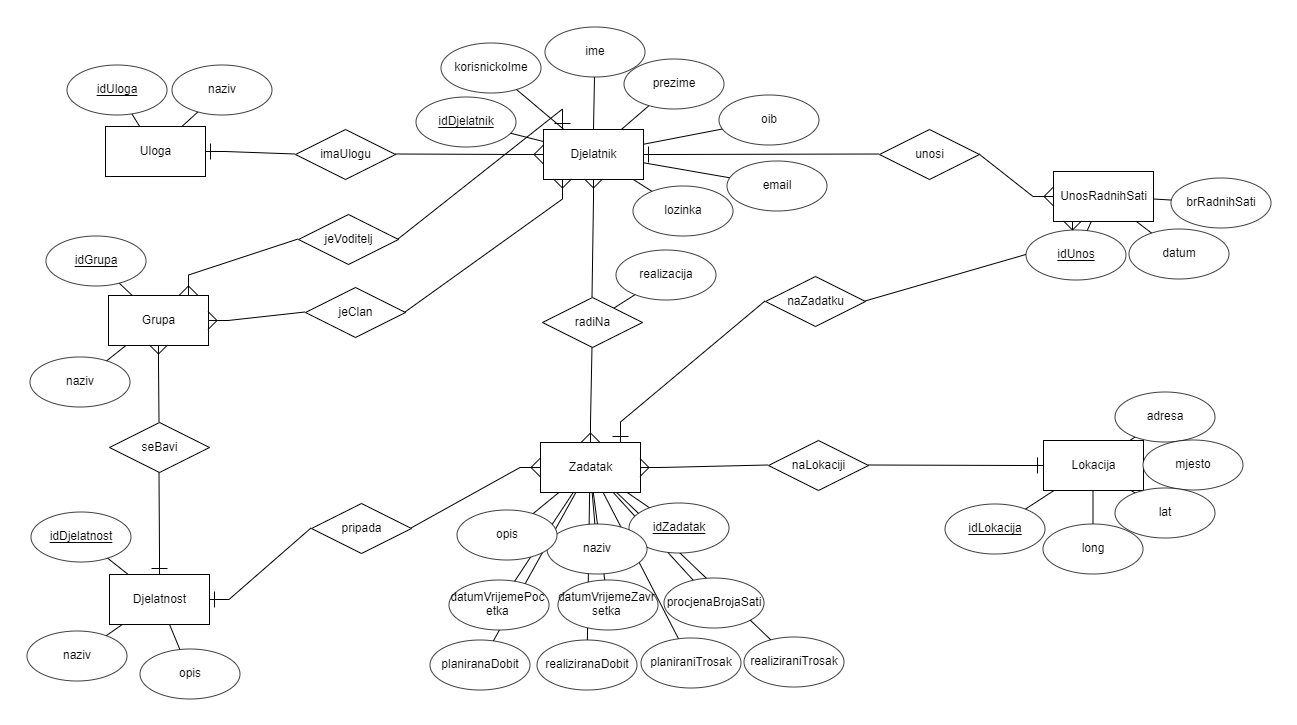
\includegraphics[width=\textwidth]{slike/ERdijagram.png}
					\caption{ER dijagram baze podataka}
				\end{figure}
			
				\begin{figure}[H]
					\centering
					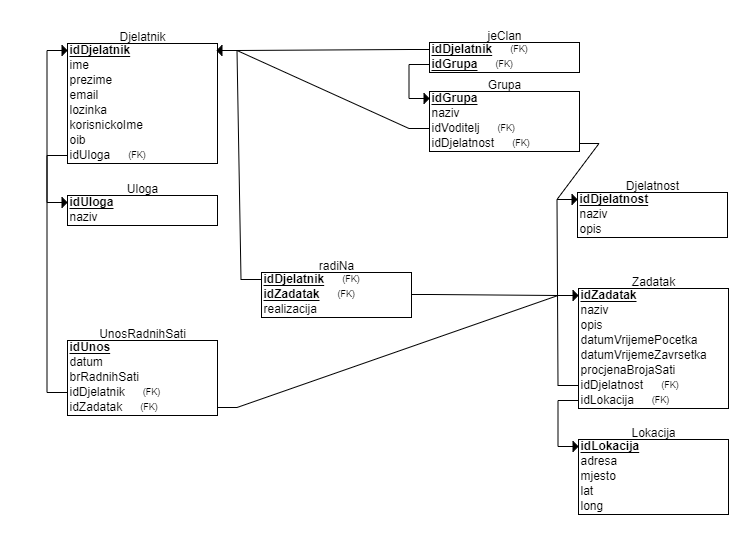
\includegraphics[width=\textwidth]{slike/RelDijagram.png}
					\caption{Relacijski dijagram baze podataka}
				\end{figure}		
			\eject
			
			
		\section{Dijagram razreda}
		
			\textit{Potrebno je priložiti dijagram razreda s pripadajućim opisom. Zbog preglednosti je moguće dijagram razlomiti na više njih, ali moraju biti grupirani prema sličnim razinama apstrakcije i srodnim funkcionalnostima.}\\
			
			\textbf{\textit{dio 1. revizije}}\\
			
			\textit{Prilikom prve predaje projekta, potrebno je priložiti potpuno razrađen dijagram razreda vezan uz \textbf{generičku funkcionalnost} sustava. Ostale funkcionalnosti trebaju biti idejno razrađene u dijagramu sa sljedećim komponentama: nazivi razreda, nazivi metoda i vrste pristupa metodama (npr. javni, zaštićeni), nazivi atributa razreda, veze i odnosi između razreda.}\\
			
			\textbf{\textit{dio 2. revizije}}\\			
			
			\textit{Prilikom druge predaje projekta dijagram razreda i opisi moraju odgovarati stvarnom stanju implementacije}
			
			
			
			\eject
		
		\section{Dijagram stanja}
			
			
			\textbf{\textit{dio 2. revizije}}\\
			
			\textit{Potrebno je priložiti dijagram stanja i opisati ga. Dovoljan je jedan dijagram stanja koji prikazuje \textbf{značajan dio funkcionalnosti} sustava. Na primjer, stanja korisničkog sučelja i tijek korištenja neke ključne funkcionalnosti jesu značajan dio sustava, a registracija i prijava nisu. }
			
			
			\eject 
		
		\section{Dijagram aktivnosti}
			
			\textbf{\textit{dio 2. revizije}}\\
			
			 \textit{Potrebno je priložiti dijagram aktivnosti s pripadajućim opisom. Dijagram aktivnosti treba prikazivati značajan dio sustava.}
			
			\eject
		\section{Dijagram komponenti}
		
			\textbf{\textit{dio 2. revizije}}\\
		
			 \textit{Potrebno je priložiti dijagram komponenti s pripadajućim opisom. Dijagram komponenti treba prikazivati strukturu cijele aplikacije.}
		\chapter{Implementacija i korisničko sučelje}
		
		
		\section{Korištene tehnologije i alati}
		
			\textbf{\textit{dio 2. revizije}}
			
			 \textit{Detaljno navesti sve tehnologije i alate koji su primijenjeni pri izradi dokumentacije i aplikacije. Ukratko ih opisati, te navesti njihovo značenje i mjesto primjene. Za svaki navedeni alat i tehnologiju je potrebno \textbf{navesti internet poveznicu} gdje se mogu preuzeti ili više saznati o njima}.
			
			
			\eject 
		
	
		\section{Ispitivanje programskog rješenja}
			
			\textbf{\textit{dio 2. revizije}}\\
			
			 \textit{U ovom poglavlju je potrebno opisati provedbu ispitivanja implementiranih funkcionalnosti na razini komponenti i na razini cijelog sustava s prikazom odabranih ispitnih slučajeva. Studenti trebaju ispitati temeljnu funkcionalnost i rubne uvjete.}
	
			
			\subsection{Ispitivanje komponenti}
			\textit{Potrebno je provesti ispitivanje jedinica (engl. unit testing) nad razredima koji implementiraju temeljne funkcionalnosti. Razraditi \textbf{minimalno 6 ispitnih slučajeva} u kojima će se ispitati redovni slučajevi, rubni uvjeti te izazivanje pogreške (engl. exception throwing). Poželjno je stvoriti i ispitni slučaj koji koristi funkcionalnosti koje nisu implementirane. Potrebno je priložiti izvorni kôd svih ispitnih slučajeva te prikaz rezultata izvođenja ispita u razvojnom okruženju (prolaz/pad ispita). }
			
			
			
			\subsection{Ispitivanje sustava}
			
			 \textit{Potrebno je provesti i opisati ispitivanje sustava koristeći radni okvir Selenium\footnote{\url{https://www.seleniumhq.org/}}. Razraditi \textbf{minimalno 4 ispitna slučaja} u kojima će se ispitati redovni slučajevi, rubni uvjeti te poziv funkcionalnosti koja nije implementirana/izaziva pogrešku kako bi se vidjelo na koji način sustav reagira kada nešto nije u potpunosti ostvareno. Ispitni slučaj se treba sastojati od ulaza (npr. korisničko ime i lozinka), očekivanog izlaza ili rezultata, koraka ispitivanja i dobivenog izlaza ili rezultata.\\ }
			 
			 \textit{Izradu ispitnih slučajeva pomoću radnog okvira Selenium moguće je provesti pomoću jednog od sljedeća dva alata:}
			 \begin{itemize}
			 	\item \textit{dodatak za preglednik \textbf{Selenium IDE} - snimanje korisnikovih akcija radi automatskog ponavljanja ispita	}
			 	\item \textit{\textbf{Selenium WebDriver} - podrška za pisanje ispita u jezicima Java, C\#, PHP koristeći posebno programsko sučelje.}
			 \end{itemize}
		 	\textit{Detalji o korištenju alata Selenium bit će prikazani na posebnom predavanju tijekom semestra.}
			
			\eject 
		
		
		\section{Dijagram razmještaja}
			
			\textbf{\textit{dio 2. revizije}}
			
			 \textit{Potrebno je umetnuti \textbf{specifikacijski} dijagram razmještaja i opisati ga. Moguće je umjesto specifikacijskog dijagrama razmještaja umetnuti dijagram razmještaja instanci, pod uvjetom da taj dijagram bolje opisuje neki važniji dio sustava.}
			
			\eject 
		
		\section{Upute za puštanje u pogon}
		
			\textbf{\textit{dio 2. revizije}}\\
		
			 \textit{U ovom poglavlju potrebno je dati upute za puštanje u pogon (engl. deployment) ostvarene aplikacije. Na primjer, za web aplikacije, opisati postupak kojim se od izvornog kôda dolazi do potpuno postavljene baze podataka i poslužitelja koji odgovara na upite korisnika. Za mobilnu aplikaciju, postupak kojim se aplikacija izgradi, te postavi na neku od trgovina. Za stolnu (engl. desktop) aplikaciju, postupak kojim se aplikacija instalira na računalo. Ukoliko mobilne i stolne aplikacije komuniciraju s poslužiteljem i/ili bazom podataka, opisati i postupak njihovog postavljanja. Pri izradi uputa preporučuje se \textbf{naglasiti korake instalacije uporabom natuknica} te koristiti što je više moguće \textbf{slike ekrana} (engl. screenshots) kako bi upute bile jasne i jednostavne za slijediti.}
			
			
			 \textit{Dovršenu aplikaciju potrebno je pokrenuti na javno dostupnom poslužitelju. Studentima se preporuča korištenje neke od sljedećih besplatnih usluga: \href{https://aws.amazon.com/}{Amazon AWS}, \href{https://azure.microsoft.com/en-us/}{Microsoft Azure} ili \href{https://www.heroku.com/}{Heroku}. Mobilne aplikacije trebaju biti objavljene na F-Droid, Google Play ili Amazon App trgovini.}
			
			
			\eject 
		\chapter{Zaključak i budući rad}
		
% 		\textbf{\textit{dio 2. revizije}}\\
		
% 		 \textit{U ovom poglavlju potrebno je napisati osvrt na vrijeme izrade projektnog zadatka, koji su tehnički izazovi prepoznati, jesu li riješeni ili kako bi mogli biti riješeni, koja su znanja stečena pri izradi projekta, koja bi znanja bila posebno potrebna za brže i kvalitetnije ostvarenje projekta i koje bi bile perspektive za nastavak rada u projektnoj grupi.}
		
% 		 \textit{Potrebno je točno popisati funkcionalnosti koje nisu implementirane u ostvarenoj aplikaciji.}

        Zadatak našega tima bio je razvoj aplikacije koja bi omogućila poduzeću „Mi puno radimo“ praćenje realizacije zadataka te raspoloživosti djelatnika kako bi se olakšala organizacija djelatnosti i zaposlenika unutar firme. Kroz 15 tjedana razvoja uspješno smo ostvarili naš cilj.  

Prvi zadatak, okupljanje tima nije bio težak. Prethodna poznanstva uvelike su olakšala komunikaciju i pozitivno pridonijele funkcioniranju grupe. Zatim je uslijedila prva faza provedbe projekta. Zajednički smo pisali dokumentaciju što je olakšalo daljnji rad. Dokumentirani zahtjevi, izrađeni obrasci i dijagrami detaljno su prikazivali željene funkcionalnosti aplikacije. Svaki član tima, na temelju priloženog, znao je točno što treba implementirati te što je već bilo odrađeno. Konkretnu implementaciju zadataka možemo svrstati u drugu fazu razvoja. 

Početak je bio težak, no zajedničkim snagama uspjeli smo se uhodati u razvoj aplikacije. Grupa se podijelila na četiri \textit{backend} programera, dva \textit{frontend} te jednog zaduženog za bazu podataka. Daljnjim razvojem i obavljanjem nekih od poslova, potreba za reorganiziranjem tima bila je nužna, stoga spomenute pozicije nisu bile fiksne cijelo vrijeme razvoja. Završna situacija zahtijevala je više \textit{frontend} programera te nekoliko osoba za sređivanje dokumentacije. Ovakva reorganizacija tima pridonijela je da svaki člana nauči više. Ipak, reorganizacijom izgubili smo dosta vremena učeći nove alate i određene jezike, ali upravo se zato možemo još više ponositi postignutim ciljem. 

Za sve članove ovakav projekt bio je potpuno novo iskustvo.  Možemo istaknuti nova stečena znanja iz programiranja, no i usvojene vještine poput rada u timu, organizacije tima, ali i vremena. Prostor za poboljšanje uvijek postoji, no svakim sljedećim ovakvim iskušenjem uslijedit će i rast našeg iskustva, te će aplikacije biti bolje. 
		
		\eject 
		\chapter*{Popis literature}
		\addcontentsline{toc}{chapter}{Popis literature}
	 	
 		\textbf{\textit{Kontinuirano osvježavanje}}
	
		\textit{Popisati sve reference i literaturu koja je pomogla pri ostvarivanju projekta.}
		
		
		\begin{enumerate}
			
			
			\item  Programsko inženjerstvo, FER ZEMRIS, \url{http://www.fer.hr/predmet/proinz}
			
			\item  I. Sommerville, "Software engineering", 8th ed, Addison Wesley, 2007.
			
			\item  T.C.Lethbridge, R.Langaniere, "Object-Oriented Software Engineering", 2nd ed. McGraw-Hill, 2005.
			
			\item  I. Marsic, Software engineering book``, Department of Electrical and Computer Engineering, Rutgers University, \url{http://www.ece.rutgers.edu/~marsic/books/SE}
			
			\item  The Unified Modeling Language, \url{https://www.uml-diagrams.org/}
			
			\item  Astah Community, \url{http://astah.net/editions/uml-new}
			
			\item  Lucidchart : Intelligent Diagramming,  \url{https://www.lucidchart.com/pages/ }
			
			\item  Tutorial: Intro to React,  \url{https://reactjs.org/tutorial/tutorial.html}
			
		\end{enumerate}
		
		 
		
		
		\begingroup
		\renewcommand*\listfigurename{Indeks slika i dijagrama}
		%\renewcommand*\listtablename{Indeks tablica}
		%\let\clearpage\relax
		\listoffigures
		%\vspace{10mm}
		%\listoftables
		\endgroup
		\addcontentsline{toc}{chapter}{Indeks slika i dijagrama}
		
		
		
		\eject 
		
		\chapter*{Dodatak: Prikaz aktivnosti grupe}
		\addcontentsline{toc}{chapter}{Dodatak: Prikaz aktivnosti grupe}
		
		\section*{Dnevnik sastajanja}
		
		\begin{packed_enum}
			\item  sastanak
			
			\item[] \begin{packed_item}
				\item Datum: 13. listopada 2021.
				\item Prisustvovali: B.Kazazić, M.Erlić, B.Pavlović, A.Pašalić, L.Raspudić, P.Sušac, V.Žunar
				\item Teme sastanka:
				\begin{packed_item}
					\item 1. sastanak s asistentom i demonstratorom
					\item raščišćavanje nejasnoća
				\end{packed_item}
			\end{packed_item}
			
			\item  sastanak
			\item[] \begin{packed_item}
				\item Datum: 14. listopada 2021.
				\item Prisustvovali: B.Kazazić, M.Erlić, B.Pavlović, A.Pašalić, L.Raspudić, V.Žunar
				\item Teme sastanka:
				\begin{packed_item}
					\item ažuriranje LaTeX dokumentacije
					\item dodjela zadataka članovima tima
					\item platforme za komunikaciju
				\end{packed_item}
			\end{packed_item}
			
			\item  sastanak
			\item[] \begin{packed_item}
				\item Datum: 18. listopada 2021.
				\item Prisustvovali: B.Kazazić, M.Erlić, B.Pavlović, L.Raspudić, P.Sušac, V.Žunar
				\item Teme sastanka:
				\begin{packed_item}
					\item raspodjela zadataka
				\end{packed_item}
			\end{packed_item}
			
			\item  sastanak
			\item[] \begin{packed_item}
				\item Datum: 22. listopada 2021.
				\item Prisustvovali: B.Kazazić, M.Erlić, B.Pavlović, A.Pašalić, P.Sušac, V.Žunar
				\item Teme sastanka:
				\begin{packed_item}
					\item dodjela zadataka članovima tima
				\end{packed_item}
			\end{packed_item}
			%
			
		\end{packed_enum}
		
		\eject
		\section*{Tablica aktivnosti}
		
			\textbf{\textit{Kontinuirano osvježavanje}}\\
			
			 \textit{Napomena: Doprinose u aktivnostima treba navesti u satima po članovima grupe po aktivnosti.}
					
						
			
			\begin{longtabu} to \textwidth {|X[7, l]|X[1, c]|X[1, c]|X[1, c]|X[1, c]|X[1, c]|X[1, c]|X[1, c]|}
								
				\cline{2-8} \multicolumn{1}{c|}{\textbf{}} &     \multicolumn{1}{c|}{\rotatebox{90}{\textbf{Bernard Kazazić }}} & \multicolumn{1}{c|}{\rotatebox{90}{\textbf{Marijan Erlić }}} &	\multicolumn{1}{c|}{\rotatebox{90}{\textbf{Barbara Pavlović }}} &	\multicolumn{1}{c|}{\rotatebox{90}{\textbf{Ante Pašalić }}} &
				\multicolumn{1}{c|}{\rotatebox{90}{\textbf{Luka Raspudić }}} &
				\multicolumn{1}{c|}{\rotatebox{90}{\textbf{Petar Sušac }}} &	\multicolumn{1}{c|}{\rotatebox{90}{\textbf{Veronika Žunar }}} \\ \hline 
				\endfirsthead
				
			
				\cline{2-8} \multicolumn{1}{c|}{\textbf{}} &     \multicolumn{1}{c|}{\rotatebox{90}{\textbf{Bernard Kazazić}}} & \multicolumn{1}{c|}{\rotatebox{90}{\textbf{Marijan Erlić }}} &	\multicolumn{1}{c|}{\rotatebox{90}{\textbf{Barbara Pavlović }}} &
				\multicolumn{1}{c|}{\rotatebox{90}{\textbf{Ante Pašalić }}} &	\multicolumn{1}{c|}{\rotatebox{90}{\textbf{Luka Raspudić }}} &
				\multicolumn{1}{c|}{\rotatebox{90}{\textbf{Petar Sušac }}} &	\multicolumn{1}{c|}{\rotatebox{90}{\textbf{Veronika Žunar }}} \\ \hline 
				\endhead
				
				
				\endfoot
							
				 
				\endlastfoot
				
				Upravljanje projektom 		&  &  &  &  &  &  & \\ \hline
				Opis projektnog zadatka 	&  &  &  &  &  &  & \\ \hline
				
				Funkcionalni zahtjevi       &  &  &  &  &  &  &  \\ \hline
				Opis pojedinih obrazaca 	&  &  &  &  &  &  &  \\ \hline
				Dijagram obrazaca 			&  &  &  &  &  &  &  \\ \hline
				Sekvencijski dijagrami 		&  &  &  &  &  &  &  \\ \hline
				Opis ostalih zahtjeva 		&  &  &  &  & 60 &  &  \\ \hline

				Arhitektura i dizajn sustava	 &  &  &  &  &  &  &  \\ \hline
				Baza podataka				&  &  &  &  &  &  &   \\ \hline
				Dijagram razreda 			&  &  &  &  &  &  &   \\ \hline
				Dijagram stanja				&  &  &  &  &  &  &  \\ \hline
				Dijagram aktivnosti 		&  &  &  &  &  &  &  \\ \hline
				Dijagram komponenti			&  &  &  &  &  &  &  \\ \hline
				Korištene tehnologije i alati 		&  &  &  &  &  &  &  \\ \hline
				Ispitivanje programskog rješenja 	&  &  &  &  &  &  &  \\ \hline
				Dijagram razmještaja			&  &  &  &  &  &  &  \\ \hline
				Upute za puštanje u pogon 		&  &  &  &  &  &  &  \\ \hline 
				Dnevnik sastajanja 			&  &  &  &  & 120 &  &  \\ \hline
				Zaključak i budući rad 		&  &  &  &  &  &  &  \\  \hline
				Popis literature 			&  &  &  &  &  &  &  \\  \hline
				&  &  &  &  &  &  &  \\ \hline \hline
				\textit{Dodatne stavke kako ste podijelili izradu aplikacije} 			&  &  &  &  &  &  &  \\ \hline
				\textit{npr. izrada početne stranice} 				&  &  &  &  &  &  &  \\ \hline 
				\textit{izrada baze podataka} 		 			&  &  &  &  &  &  & \\ \hline 
				\textit{spajanje s bazom podataka} 							&  &  &  &  &  &  &  \\ \hline
				\textit{back end} 							&  &  &  &  &  &  &  \\  \hline
				 							&  &  &  &  &  &  &\\  \hline
				
				
			\end{longtabu}
					
					
		\eject
		\section*{Dijagrami pregleda promjena}
		
		\textbf{\textit{dio 2. revizije}}\\
		
		\textit{Prenijeti dijagram pregleda promjena nad datotekama projekta. Potrebno je na kraju projekta generirane grafove s gitlaba prenijeti u ovo poglavlje dokumentacije. Dijagrami za vlastiti projekt se mogu preuzeti s gitlab.com stranice, u izborniku Repository, pritiskom na stavku Contributors.}
		
	
		
		
	\end{document} %naredbe i tekst nakon ove naredbe ne ulaze u izgrađen dokument 
	
	
